\documentclass[11pt]{article}

\usepackage[utf8]{inputenc}
\usepackage[T1]{fontenc}
\usepackage{lmodern}
\usepackage{microtype}
\usepackage{amsmath,amssymb}
\usepackage{booktabs}
\usepackage{multirow}
\usepackage{algorithm}
\usepackage{algpseudocode}
\usepackage{tikz}
\usetikzlibrary{positioning,arrows.meta}
\usepackage{graphicx}
\usepackage{hyperref}
\usepackage{geometry}
\geometry{margin=1in}

\title{LineDraw:
Converting Spectrograms into Sparse Musical Tokens}
\author{BoYu Wang}
\date{}

% 追踪“相对显著性”
% Spectral Saliency

% 本文提出一种 octave-normalized spectrogram
% 并基于此构建 sparse line representation

\begin{document}

\maketitle

\begin{abstract}
We propose LineDraw,
    a signal-processing-based framework
    that represents audio
    as a collection of sparse line events in the time-frequency domain.
Unlike neural approaches such as DDSP,
    LineDraw does not rely on learned parameters.
Instead, it extracts continuous frequency trajectories
    from normalized multi-window CQT representations and
    reconstructs audio through sinusoidal synthesis.
Experimental results demonstrate that
    the extracted line representation preserves both musical note information
    and spectral structure.
We further discuss its potential applications in music language modeling,
    audio understanding, and large-scale self-supervised music learning.
% 中文：我们提出了 LineDraw，这是一种基于信号处理的框架，可将音频表示为时频域中的稀疏线事件集合。
% 不同于 DDSP 等神经方法，LineDraw 不依赖学习得到的参数。
% 相反，它从归一化的多窗 CQT 表示中提取连续频率轨迹，并通过正弦合成重建音频。
% 实验结果表明，所提取的线表示能够同时保留音乐音符信息与频谱结构。
% 我们进一步讨论了其在音乐语言建模、音频理解和大规模自监督音乐学习中的潜在应用。

\end{abstract}

\section{Introduction}
Audio is highly structured,
    and many musical events appear as continuous trajectories
    in the time-frequency domain.
Current neural approaches often model audio as dense tensors.
We investigate whether a sparse line representation
    can provide a simpler and more interpretable alternative.
% 中文：音频具有很强的结构性，许多音乐事件在时频域中表现为连续轨迹。
% 当前神经方法通常将音频建模为稠密张量。
% 我们研究稀疏线表示是否能够提供更简单且更可解释的替代方案。

\section{Related Work}
\subsection{Sinusoidal Modeling}
% TODO: summarize classical sinusoidal analysis/synthesis.

\subsection{Spectral Modeling Synthesis}
% TODO: discuss SMS and relevance to trajectory modeling.

\subsection{DDSP and Neural Audio Synthesis}
% TODO: compare parameterized neural synthesis with non-parametric LineDraw.

DDSP:
audio = neural network + sinusoidal/noise synthesizer
% 中文：DDSP：音频 = 神经网络 + 正弦/噪声合成器。

LineDraw:
audio = signal processing + line extraction + sinusoidal/noise synthesizer
% 中文：LineDraw：音频 = 信号处理 + 线提取 + 正弦/噪声合成器。

\subsection{AMT and Sparse Coding}
% TODO: connect note extraction and sparse representations.

\section{Method}

\begin{figure*}[htbp]
    \centering

    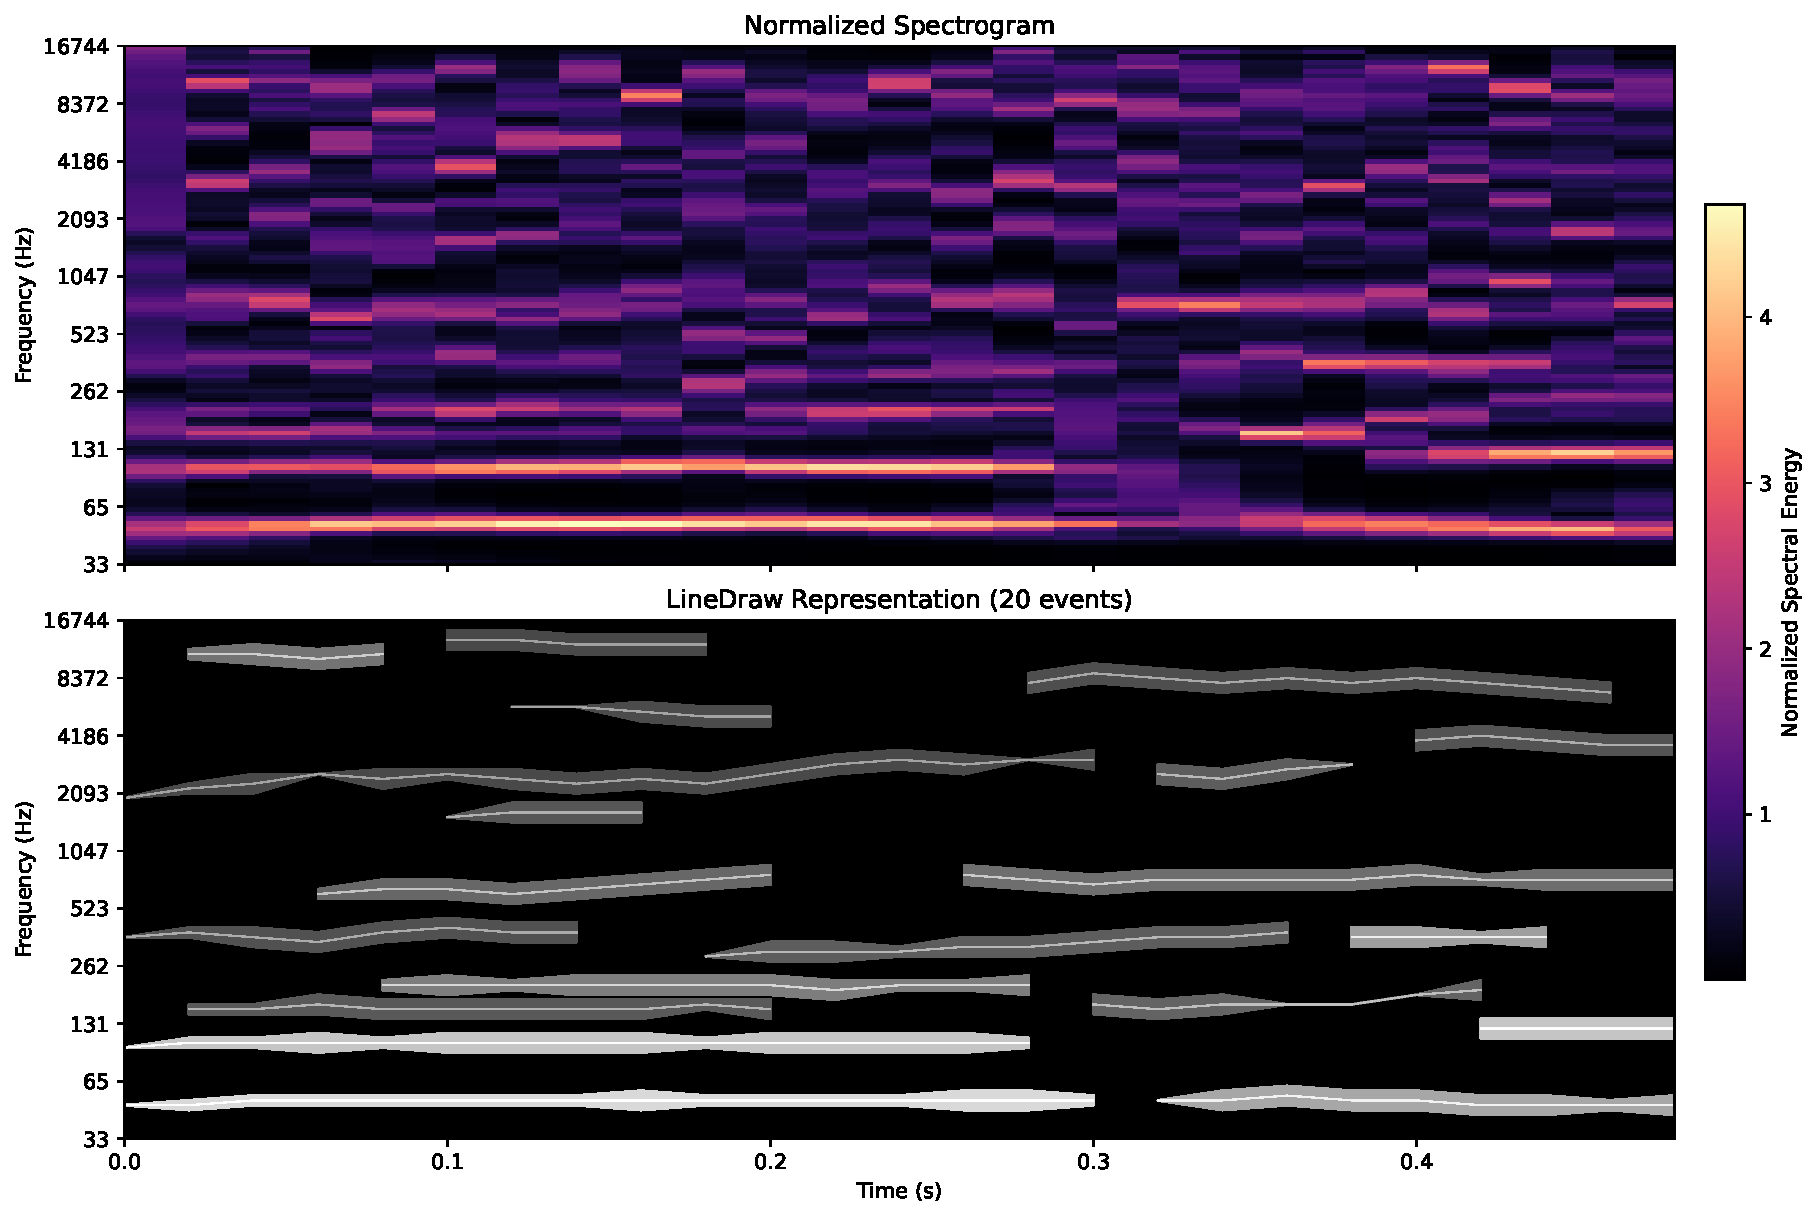
\includegraphics[width=0.32\linewidth]{../visualize/line0.pdf}
    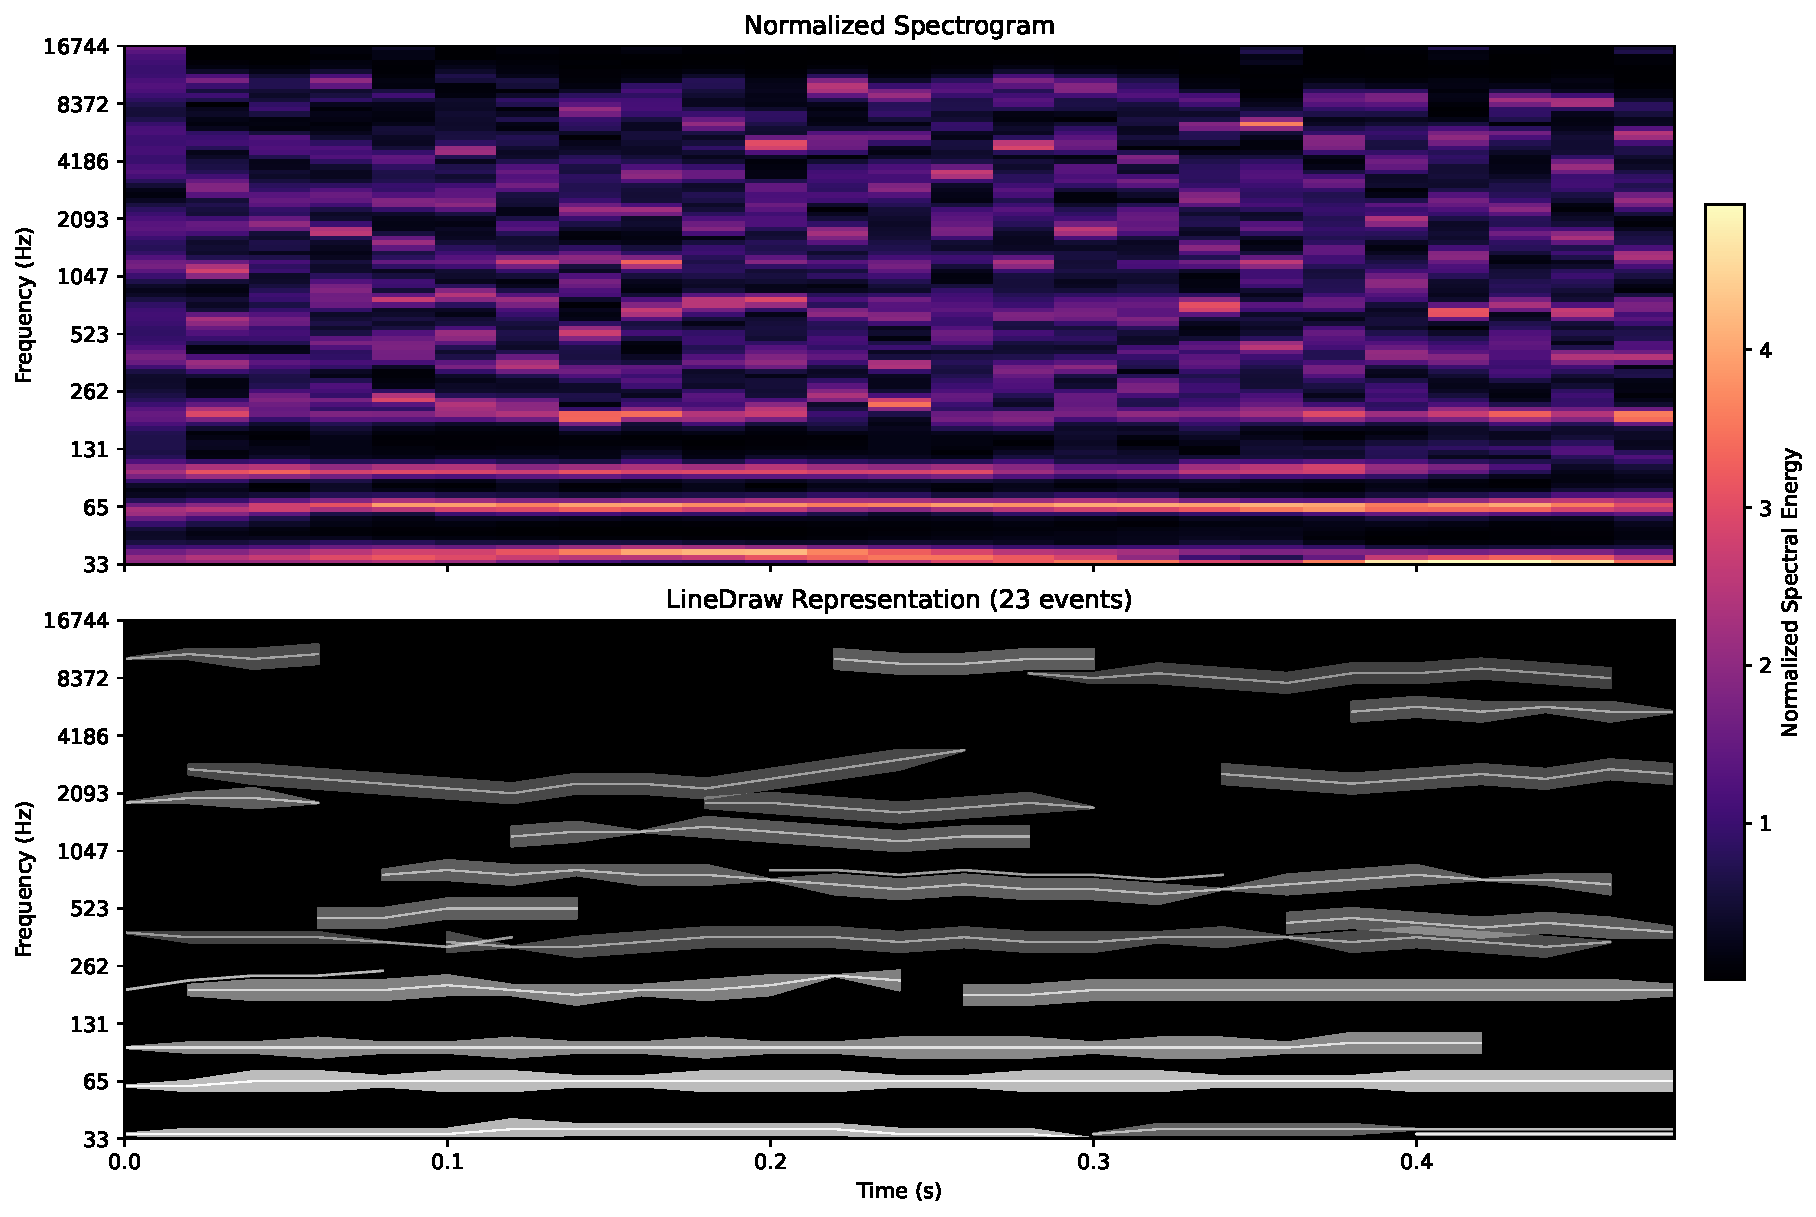
\includegraphics[width=0.32\linewidth]{../visualize/line1.pdf}
    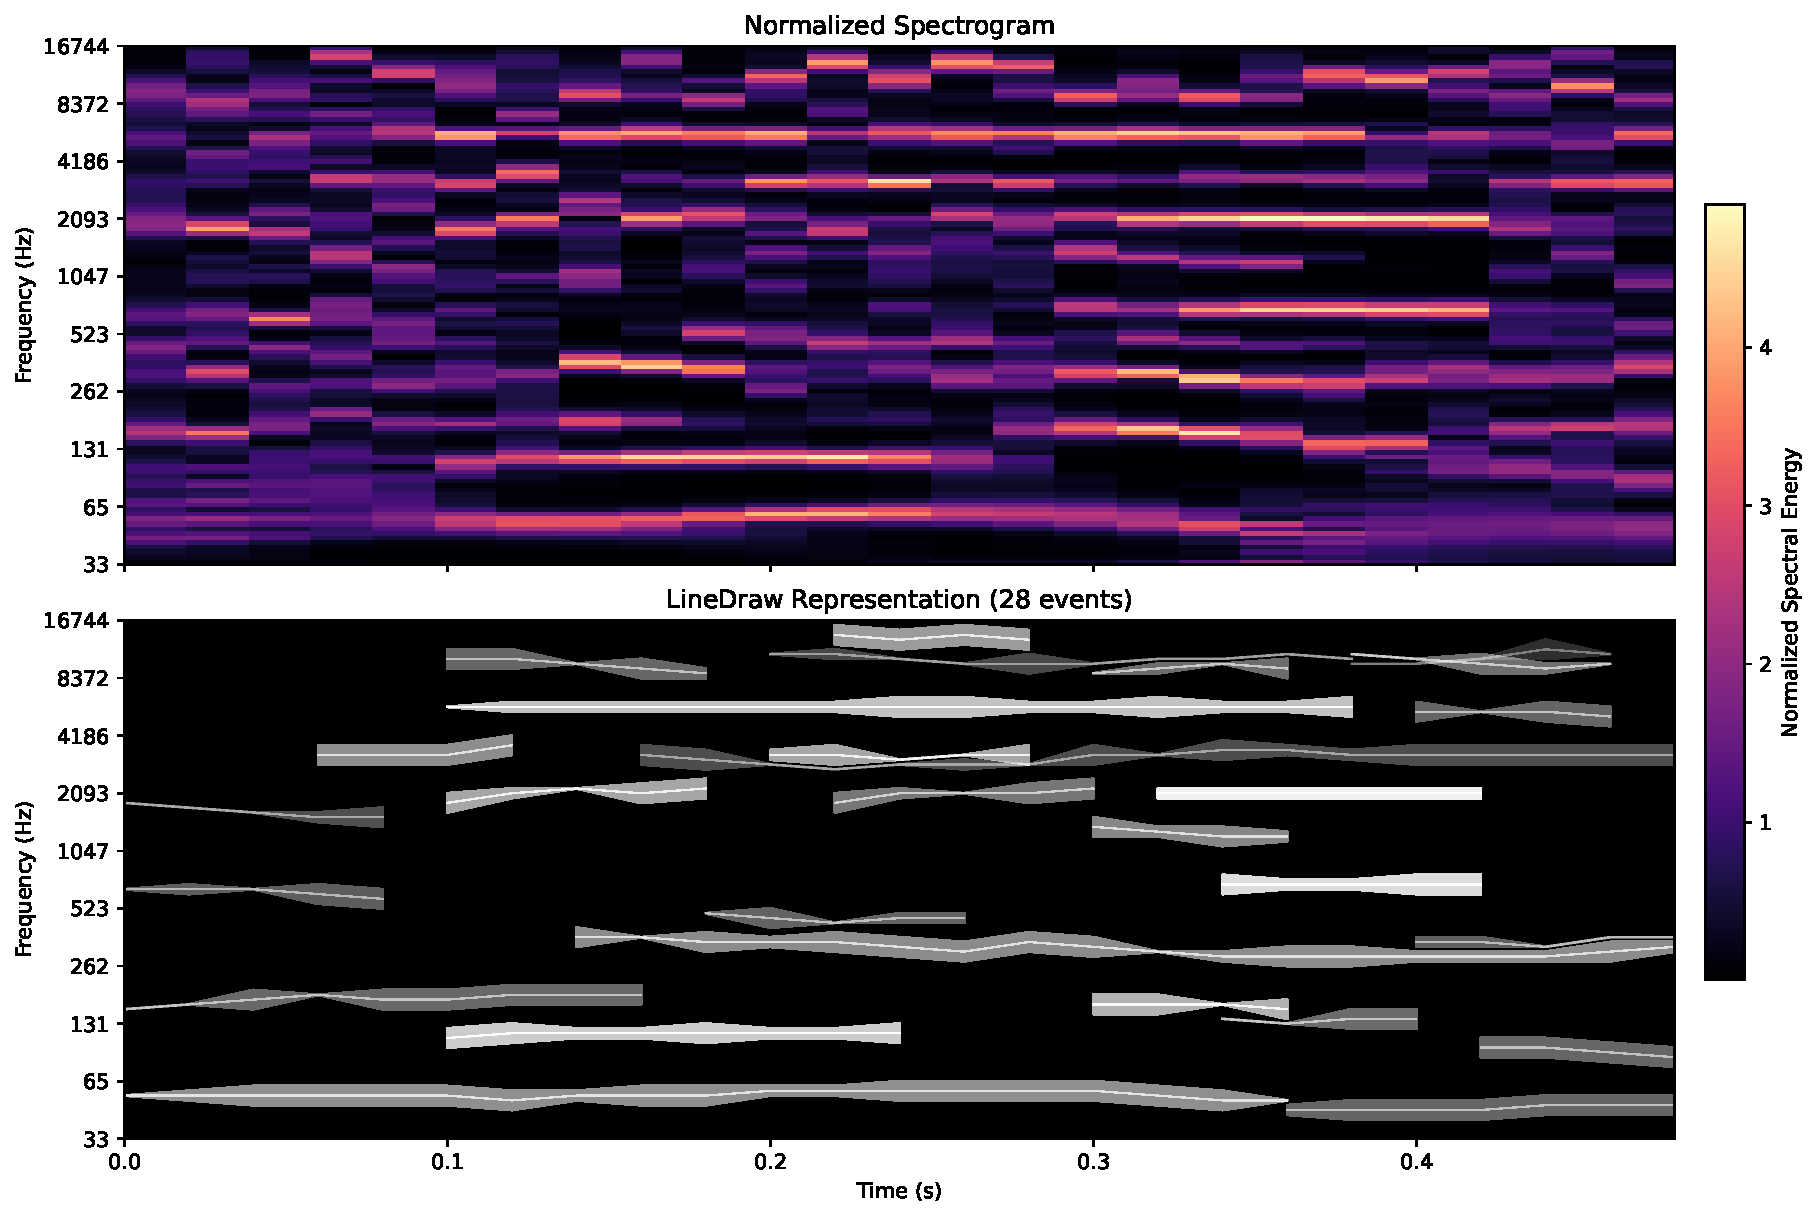
\includegraphics[width=0.32\linewidth]{../visualize/line2.pdf}

    \vspace{0.5em}

    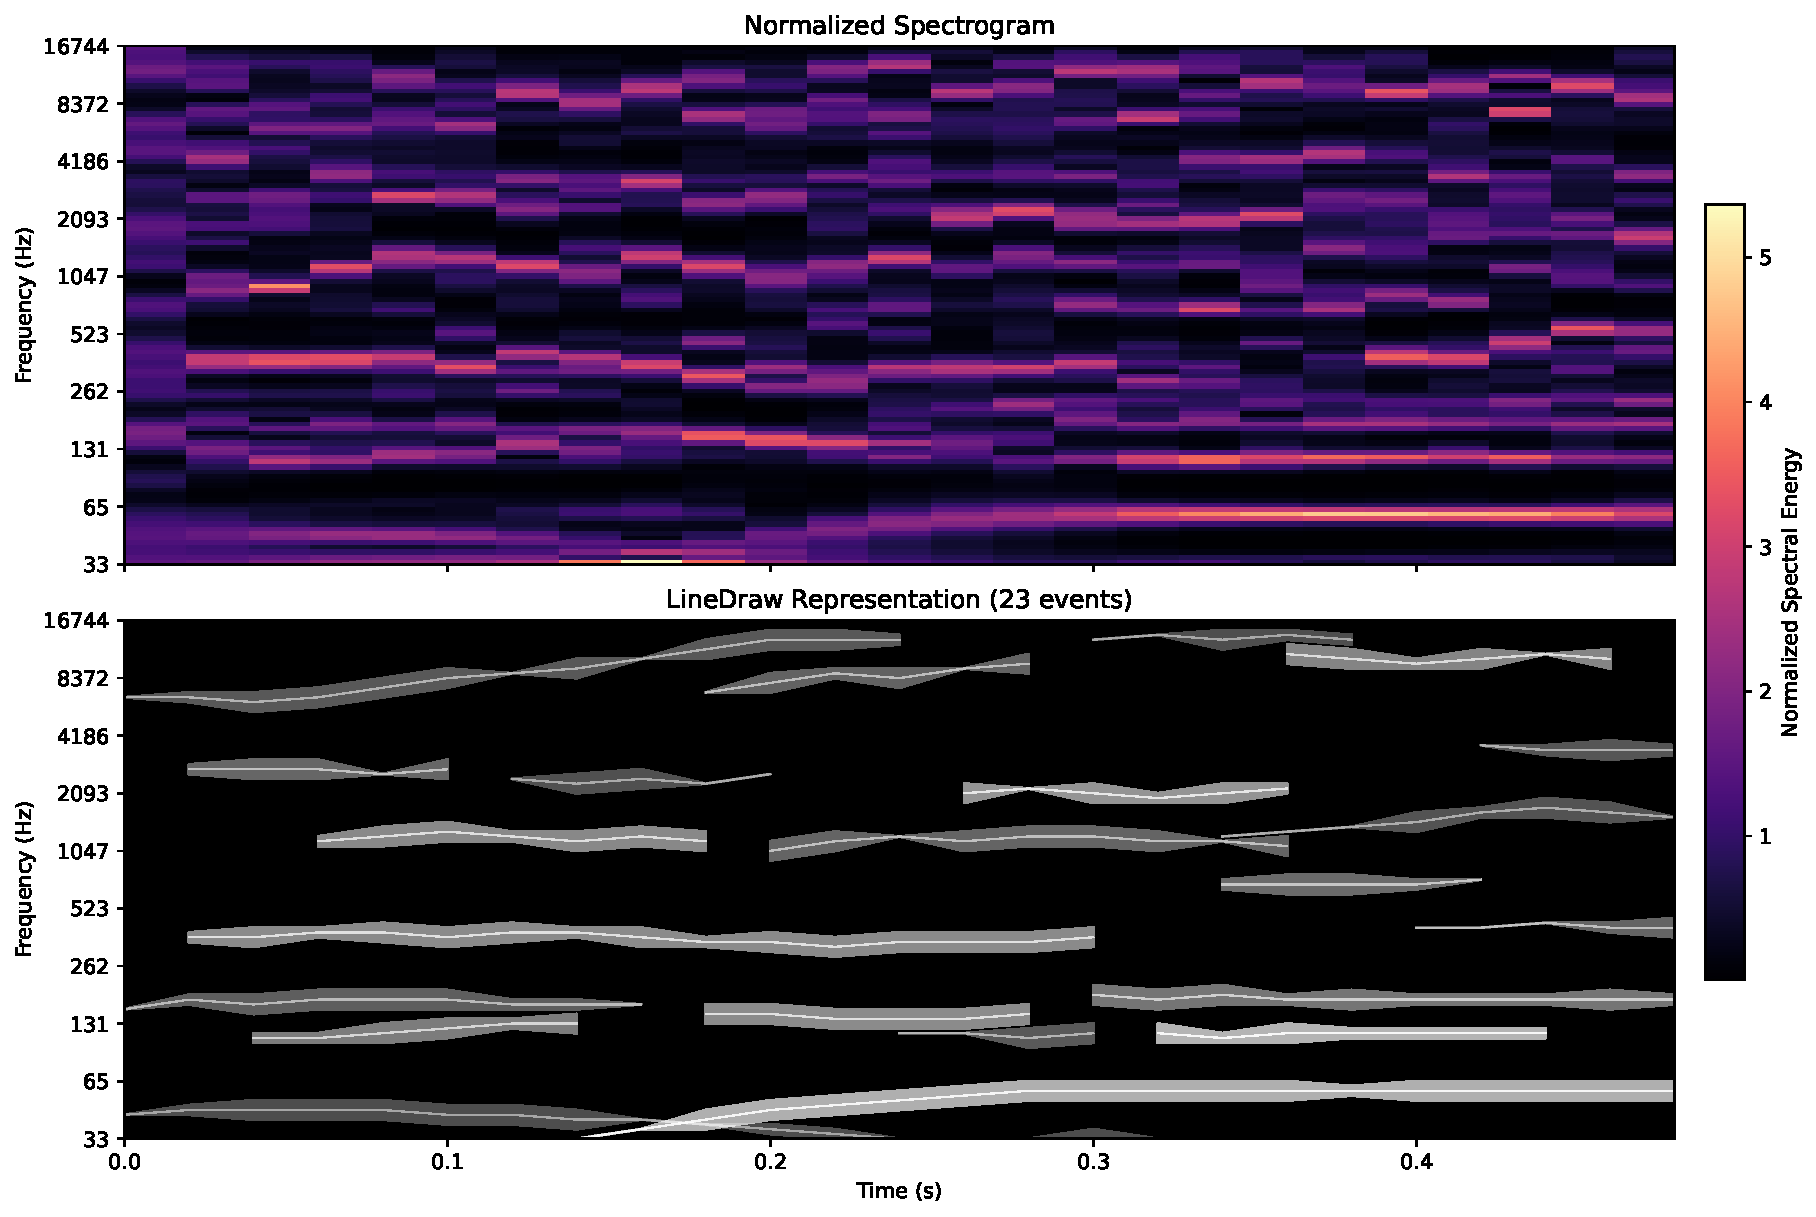
\includegraphics[width=0.32\linewidth]{../visualize/line3.pdf}
    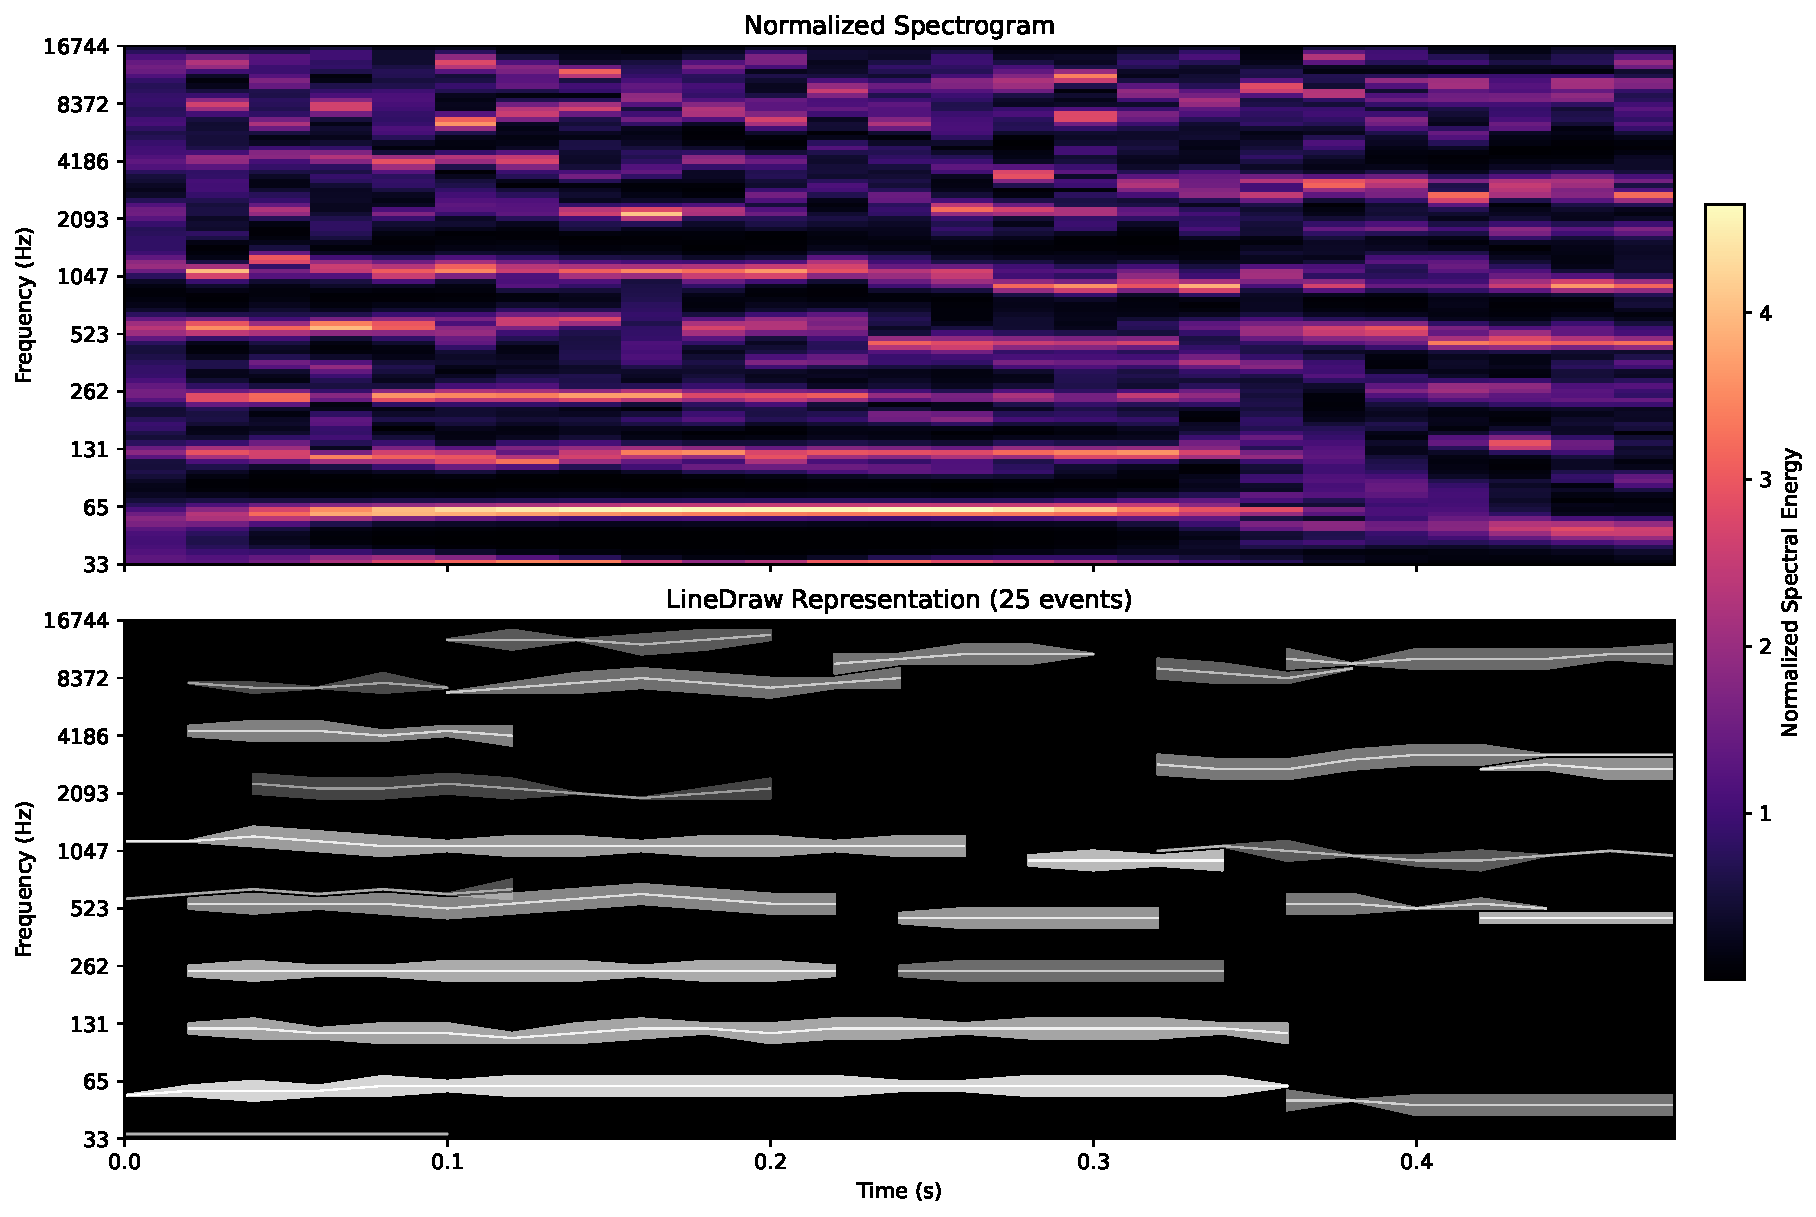
\includegraphics[width=0.32\linewidth]{../visualize/line4.pdf}
    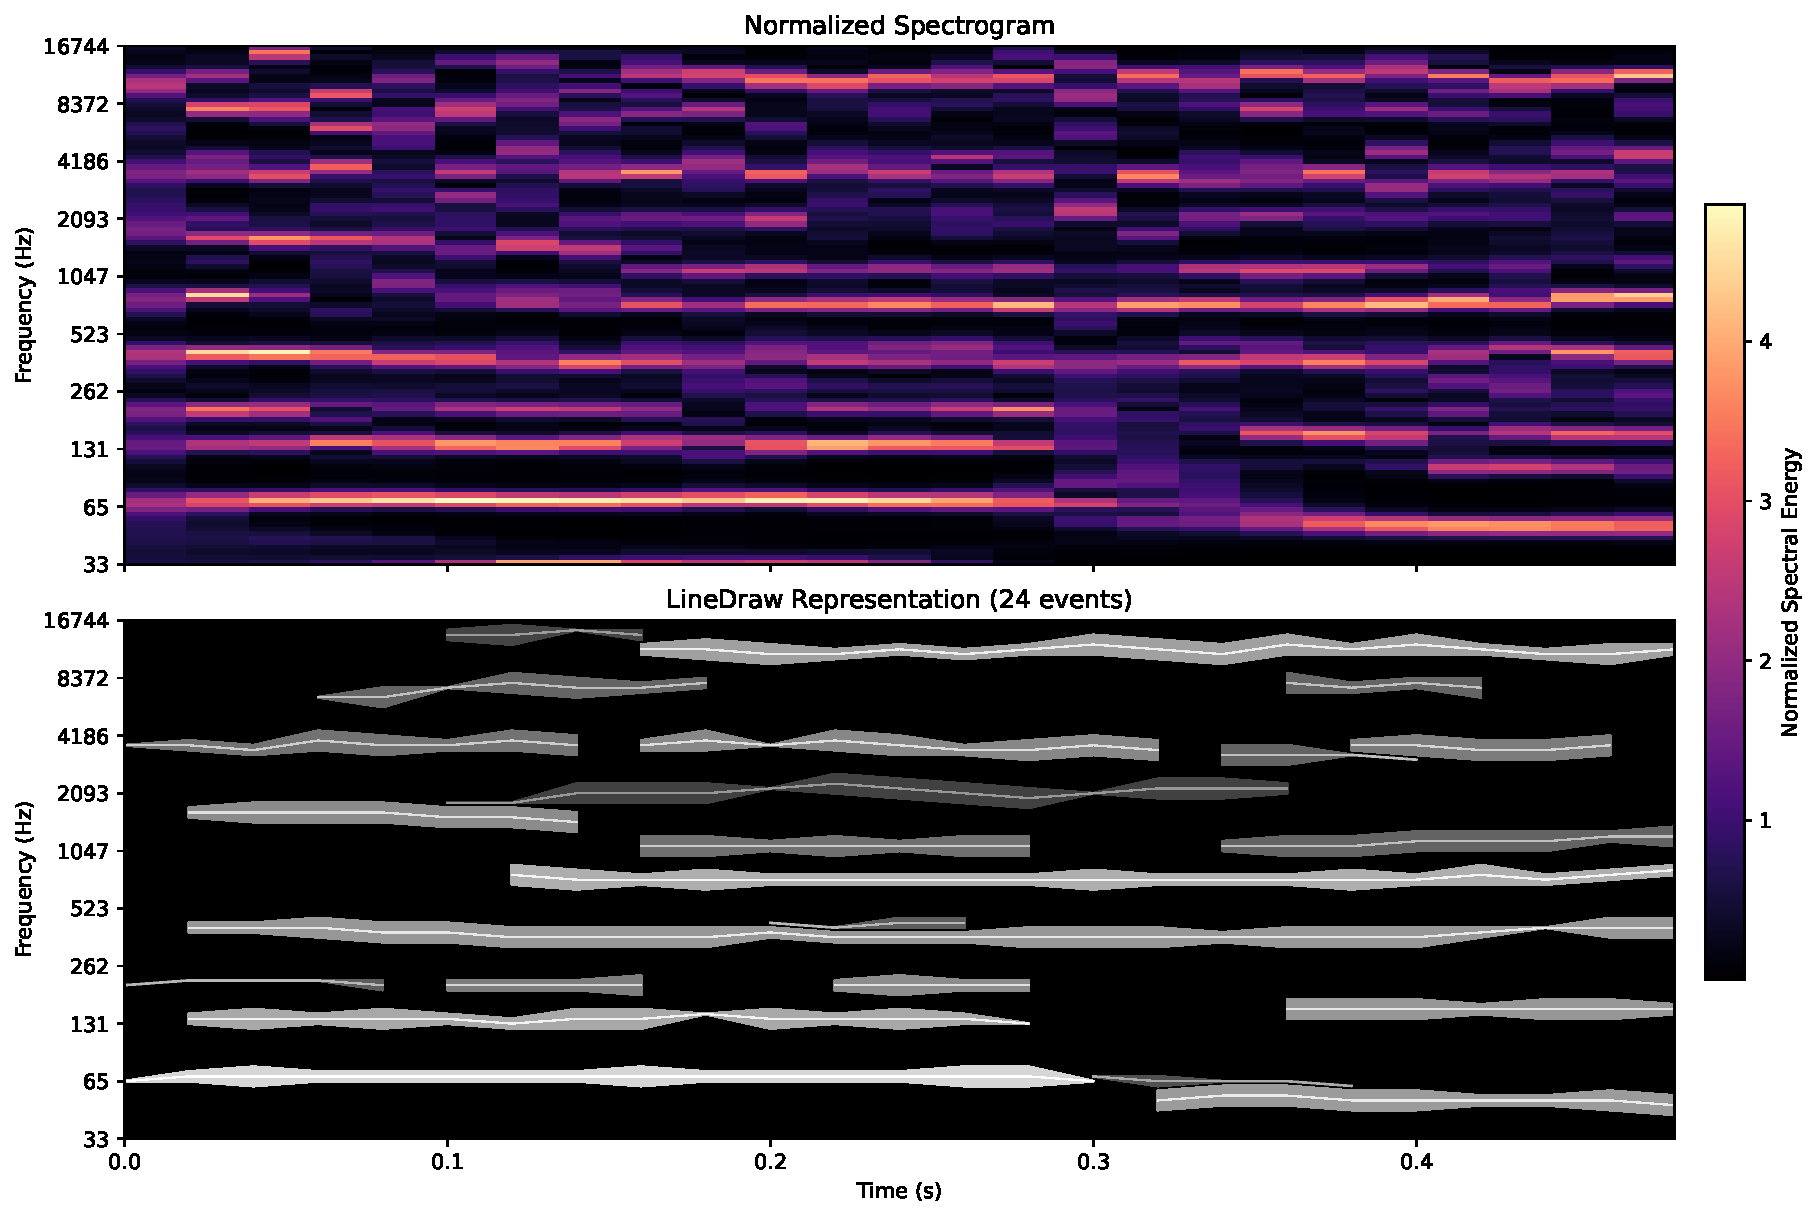
\includegraphics[width=0.32\linewidth]{../visualize/line5.pdf}

    \caption{
    Additional examples of LineDraw representations.
    % 中文：LineDraw 表示的更多示例。
    Each example shows the normalized spectrogram (top)
    % 中文：每个示例展示归一化频谱图（上）。
    and the corresponding extracted line events (bottom).
    % 中文：以及对应提取出的线事件（下）。
    The examples are randomly sampled from the evaluation dataset.
    % 中文：这些示例从评测数据集中随机采样得到。
    }
    \label{fig:linedraw_more}
\end{figure*}


% TODO:
% Contribution 1

% 提出 octave-normalized spectrogram

% Contribution 2

% 提出 LineDraw tokenization，
% 将谱图转换为稀疏线事件

% Contribution 3

% 证明这些 token 可用于

% Multi-Pitch Recognition

% Audio Resynthesis

% Future Audio-Language Modeling

% 因此，这些 token 可以用于LALM的输入，或者用于计算 RL 的 reward




\subsection{Multi-window CQT}
Given an audio signal $x(t)$, we compute a multi-window CQT stack:
% 中文：给定音频信号 $x(t)$，我们计算多窗 CQT 堆叠：
\begin{equation}
X_k(f,\tau) = \mathrm{CQT}_{w_k}\{x\}(f,\tau),
\end{equation}
where $w_k$ denotes the $k$-th analysis window.
% 中文：其中 $w_k$ 表示第 $k$ 个分析窗。

\subsection{Local Frequency Normalization}
We normalize local energy to reduce amplitude bias:
% 中文：我们对局部能量进行归一化以减小幅度偏置：
\begin{equation}
\tilde{X}(f,\tau) = \frac{X(f,\tau)}{\epsilon + \mathcal{N}(X)(f,\tau)},
\end{equation}
where $\mathcal{N}(\cdot)$ is a local neighborhood statistic and $\epsilon>0$ is a stability constant.
% 中文：其中 $\mathcal{N}(\cdot)$ 是局部邻域统计量，$\epsilon>0$ 为稳定性常数。

\subsection{Line Extraction}
Line candidates are extracted by thresholding and continuity constraints in the normalized CQT plane. A line event is defined as a connected trajectory
% 中文：在线归一化 CQT 平面中，通过阈值与连续性约束提取线候选。线事件被定义为一条连通轨迹。
\begin{equation}
\ell_i = \{(f_t, t)\}_{t=t_s}^{t_e},
\end{equation}
with minimum duration and smoothness constraints.
% 中文：并满足最小时长与平滑性约束。

\subsection{Line Event Representation}
Each line is represented as a tuple:
% 中文：每条线表示为一个元组：
\begin{equation}
e_i = (t_s, t_e, f(t), a(t), \phi_0),
\end{equation}
where $f(t)$ is instantaneous frequency, $a(t)$ is amplitude envelope, and $\phi_0$ is initial phase.
% 中文：其中 $f(t)$ 是瞬时频率，$a(t)$ 是幅度包络，$\phi_0$ 是初始相位。

\subsection{Sinusoidal Resynthesis}
Reconstruction is obtained by summing all extracted line events:
% 中文：通过对所有提取出的线事件求和得到重建信号：
\begin{equation}
\hat{x}(t) = \sum_i a_i(t)\cos\!\left(2\pi \int_0^t f_i(\tau)\,d\tau + \phi_i\right).
\end{equation}

\section{Experiments}

\subsection{Dataset Construction}

To evaluate the proposed LineDraw representation, we constructed a manually annotated pitch dataset from YouTube recordings.
% 中文：为评估所提出的 LineDraw 表示，我们基于 YouTube 录音构建了一个人工标注的音高数据集。

Audio clips were collected from a diverse set of musical sources retrieved using YouTube search. We queried multiple keywords spanning different musical styles, including popular music, piano performances, electronic dance music, jazz, orchestral music, rhythm games, and independent composers. The retrieved videos were randomly sampled and segmented into short audio excerpts.
% 中文：音频片段来自通过 YouTube 搜索获取的多样化音乐来源。我们使用覆盖不同音乐风格的多个关键词进行检索，包括流行音乐、钢琴演奏、电子舞曲、爵士、管弦乐、音游和独立作曲者。检索到的视频被随机采样并切分为短音频片段。

Each sample consists of a 0.5-second stereo audio segment sampled at 44.1 kHz. During annotation, a Constant-Q Transform (CQT) visualization was provided as an auxiliary tool to facilitate pitch labeling. Annotators were asked to identify all salient pitches present in each segment. The resulting dataset contains 1,155 annotated audio clips.
% 中文：每个样本由一个 0.5 秒、采样率 44.1 kHz 的立体声音频片段构成。标注过程中提供了常数 Q 变换（CQT）可视化作为辅助工具，以便进行音高标注。标注者需识别每个片段中所有显著音高。最终数据集包含 1,155 个已标注音频片段。

Unlike conventional Automatic Music Transcription (AMT) datasets, the proposed dataset only contains clip-level pitch annotations and does not provide note onset or offset information. Consequently, evaluation focuses on pitch presence rather than temporal note alignment.
% 中文：不同于传统自动音乐转录（AMT）数据集，该数据集仅包含片段级音高标注，不提供音符起止时间信息。因此，评估关注音高是否出现，而非音符时间对齐。

Figure~\ref{fig:dataset_statistics} summarizes the statistical properties of the dataset. The event-count distribution illustrates the number of annotated pitches per clip. The pitch-class histogram demonstrates a relatively balanced distribution among the twelve pitch classes, while the octave histogram indicates that most annotated notes concentrate in the middle musical register.
% 中文：图~\ref{fig:dataset_statistics} 总结了该数据集的统计特性。事件数分布展示了每个片段中标注音高的数量。音级直方图显示十二个音级之间分布相对均衡，而八度直方图表明多数标注音符集中在中音区。

\begin{figure*}[htbp]
\centering


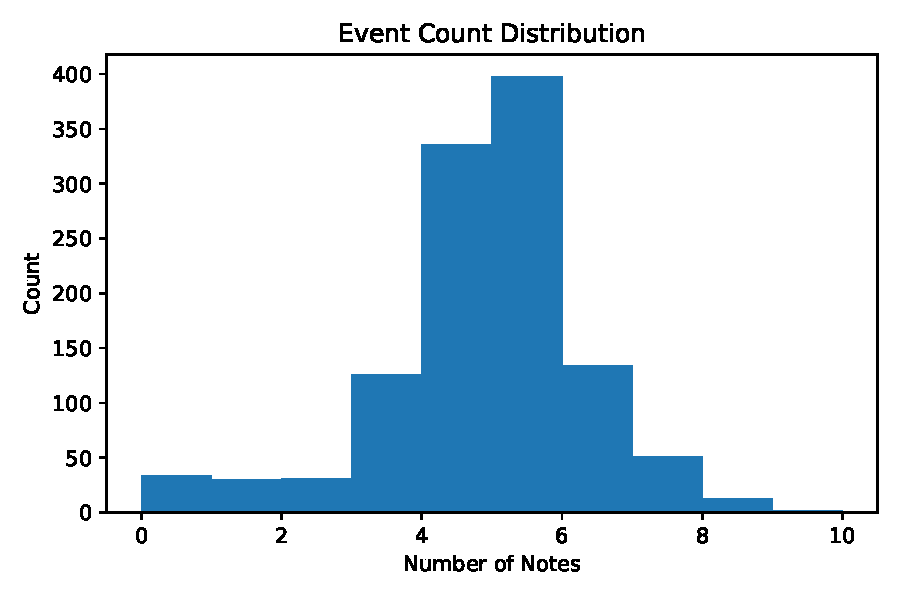
\includegraphics[width=0.32\linewidth]{../experiment/event_hist.pdf}
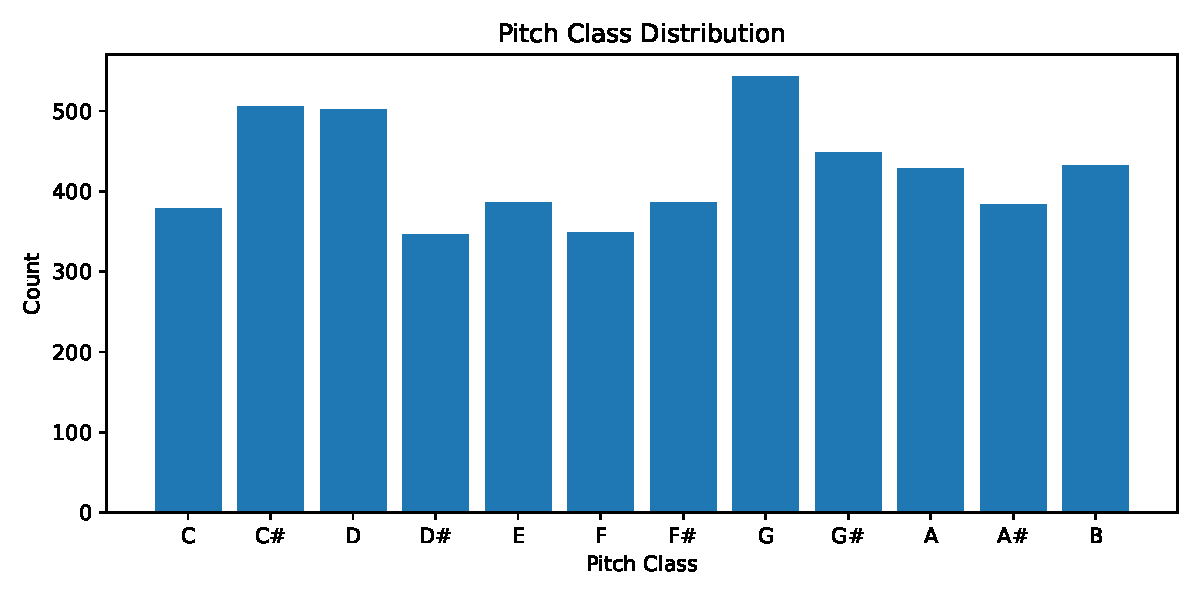
\includegraphics[width=0.32\linewidth]{../experiment/pitch_cls_hist.pdf}
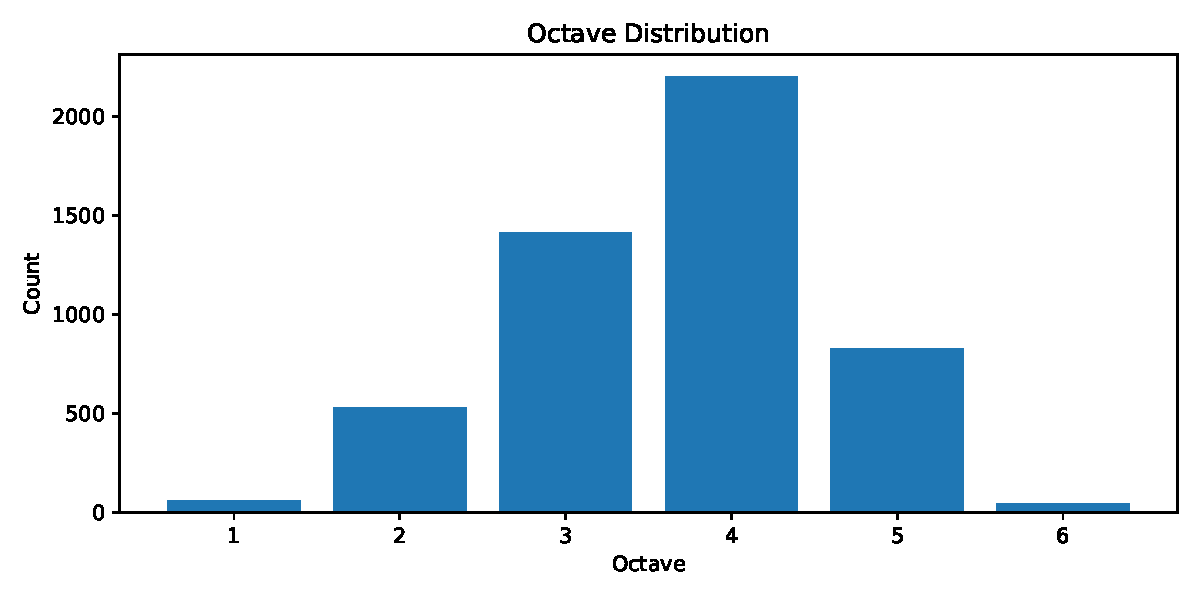
\includegraphics[width=0.32\linewidth]{../experiment/octave_hist.pdf}

\caption{
Statistical analysis of the collected pitch dataset.
% 中文：所收集音高数据集的统计分析。
Left: distribution of the number of annotated pitches per audio segment.
% 中文：左图：每个音频片段中标注音高数量的分布。
Middle: pitch-class distribution.
% 中文：中图：音级分布。
Right: octave distribution.
% 中文：右图：八度分布。
The dataset contains 1,155 manually annotated 0.5-second audio clips collected from diverse YouTube sources.
% 中文：该数据集包含 1,155 个时长 0.5 秒的人工标注音频片段，来源于多样化的 YouTube 资源。
}
\label{fig:dataset_statistics}


\end{figure*}


\subsection{Note Recovery}
\textbf{Metrics:} Precision, Recall, F1.\\
% 中文：指标：精确率、召回率、F1。
\textbf{Ground truth:} MIDI note annotations.\\
% 中文：真值：MIDI 音符标注。
\textbf{Prediction:} LineDraw note list mapped from extracted line events.
% 中文：预测：由提取线事件映射得到的 LineDraw 音符列表。

\begin{table}[htbp]
\centering
\caption{Performance of LineDraw under different extraction thresholds. ECR denotes the Explained Energy Ratio, and Events denotes the average number of extracted line events per audio clip.}
% 中文：LineDraw 在不同提取阈值下的性能。ECR 表示解释能量比，Events 表示每个音频片段平均提取出的线事件数量。
\label{tab:linedraw_threshold}

%wssb:start:linedraw_threshold
\begin{tabular}{c|ccc|ccc|cc}
\toprule
\multirow{2}{*}{Threshold}
&
\multicolumn{3}{c|}{MIDI-Level}
&
\multicolumn{3}{c|}{Pitch-Class}
&
\multirow{2}{*}{ECR $\uparrow$}
&
\multirow{2}{*}{Events $\downarrow$}
\\

&
Precision $\uparrow$
&
Recall $\uparrow$
&
F1 $\uparrow$
&
Precision $\uparrow$
&
Recall $\uparrow$
&
F1 $\uparrow$
&
&
\\
\midrule

0.7 & 0.116 & \textbf{0.794} & 0.203 & 0.273 & \textbf{0.990} & 0.428 & 0.892 & 76.75 \\

1.0 & 0.140 & 0.739 & 0.236 & 0.290 & 0.967 & 0.446 & 0.813 & 55.86 \\

2.0 & 0.233 & 0.559 & 0.329 & 0.404 & 0.837 & 0.545 & 0.543 & 20.55 \\

3.0 \textbf{Best} & 0.304 & 0.395 & \textbf{0.343} & 0.526 & 0.652 & \textbf{0.582} & 0.328 & 8.19 \\

4.0 & 0.342 & 0.213 & 0.263 & 0.631 & 0.415 & 0.501 & 0.182 & 3.19 \\

4.3 & \textbf{0.348} & 0.157 & 0.216 & \textbf{0.663} & 0.331 & 0.441 & 0.142 & \textbf{2.23} \\

\bottomrule
\end{tabular}
%wssb:end:linedraw_threshold

\end{table}

% 8个token
% 保留了58\%的音符结构。


\subsection{Spectral Reconstruction}
\textbf{Metrics:} L1 distance and MSE between reference and reconstructed spectrograms.
% 中文：指标：参考频谱与重建频谱之间的 L1 距离和 MSE。

\subsection{Threshold Analysis}
\textbf{Metrics:} ROC curve and AUC under varying extraction thresholds.
% 中文：指标：在不同提取阈值下的 ROC 曲线与 AUC。

\section{Discussion}
\subsection{Interpretability}
The line representation offers explicit event-level trajectories that are easier to inspect than dense latent tensors.
% 中文：线表示提供了显式的事件级轨迹，相比稠密潜在张量更易于检查与理解。

\subsection{Computational Cost}
% TODO: report runtime and memory comparisons with baselines.

\subsection{Failure Cases}
% TODO: analyze dense polyphony, noisy mixtures, and rapid transients.

\section{Future Work}
\subsection{Line Transformer}
Learning sequence models directly over line events.
% 中文：直接在线事件上学习序列模型。

\subsection{Audio LLM}
Using line tokens as a compact interface for multimodal audio-language reasoning.
% 中文：使用线 token 作为多模态音频-语言推理的紧凑接口。

\subsection{Large-scale Self-Supervised Learning}
Pretraining with masked line modeling and trajectory prediction.
% 中文：通过掩码线建模与轨迹预测进行预训练。

\subsection{Music Generation}
Controllable synthesis by editing line event sequences.
% 中文：通过编辑线事件序列实现可控合成。

\section{Conclusion}
LineDraw provides a sparse and interpretable audio representation based on time-frequency line extraction, with competitive note and spectral reconstruction quality and promising downstream potential.
% 中文：LineDraw 基于时频线提取提供了一种稀疏且可解释的音频表示，在音符恢复和频谱重建质量上具有竞争力，并具备良好的下游应用潜力。

% 宛如boss进入第二阶段一般震撼
\section{Draw Agent}

% 之前干的事，你就当是复现了 正弦建模 的经典工作吧
% 因为接下来，我的工作才要刚刚开始



\bibliographystyle{plain}
\bibliography{refs}

\end{document}
